\documentclass[10pt, aspectratio=169]{beamer}
\usefonttheme{professionalfonts}

\mode<presentation>
{
  \usetheme{Berkeley}
  \usecolortheme{beaver}
  \usefonttheme{default}
  \setbeamertemplate{navigation symbols}{}
  \setbeamertemplate{caption}[numbered]
} 

\setbeamertemplate{footline}{%
  \leavevmode%
  \hbox{%
    \begin{beamercolorbox}[wd=.85\paperwidth,ht=2.5ex,dp=1ex,left]{author in head/foot}%
      \usebeamerfont{author in head/foot}Maxx Seminario, Electronic Circuits, Spring 2026%
    \end{beamercolorbox}%
    \begin{beamercolorbox}[wd=.15\paperwidth,ht=2.5ex,dp=1ex,right]{date in head/foot}%
      \hspace*{0.5em}\insertframenumber{} / \inserttotalframenumber\hspace*{0.5em}%
    \end{beamercolorbox}%
  }%
  \vskip0pt%
}

\usepackage[english]{babel}
\usepackage[utf8x]{inputenc}
\usepackage{tikz}
\usetikzlibrary{shapes.geometric}
\usepackage{pgfplots}
\usepackage{array}
\usepackage{makecell}
\usepackage{verbatim}
\usepackage{graphicx}
\usepackage{subcaption}
\usepackage{amsfonts}
\usepackage{amsmath}
\usepackage{bm}
\usepackage{epstopdf}
\usepackage{circuitikz}
\usepackage{caption}
\usepackage{multirow}
\captionsetup{compatibility=false}
\usepackage[absolute,overlay]{textpos}
\usetikzlibrary{calc}
\usetikzlibrary{pgfplots.fillbetween, backgrounds}
\usetikzlibrary{positioning}
\usetikzlibrary{pgfplots.groupplots}
\usetikzlibrary{plotmarks}
\usetikzlibrary{calc}
\usepgfplotslibrary{groupplots}
\pgfplotsset{compat=newest} 

\usepackage{hyperref}
\definecolor{BeaverRed}{RGB}{179,38,38} 
\hypersetup{
    colorlinks=true,
    linkcolor=BeaverRed,
    filecolor=magenta,      
    urlcolor=cyan,
}

% Added by Maxx Seminario - for colored icons in itemize labels
\usepackage{wasysym} 
\newcommand{\neutralface}{%
  \tikz[baseline=-0.6ex]{
    \draw (0,0) circle (0.9ex);
    \fill (-0.35ex,0.25ex) circle (0.12ex);
    \fill ( 0.35ex,0.25ex) circle (0.12ex);
    \draw (-0.35ex,-0.25ex) -- (0.35ex,-0.25ex);
  }%
}

\newcommand{\baditem}{\textcolor{red! 70! black}{\frownie}}
\newcommand{\gooditem}{\textcolor{green!60!black}{\smiley}}
\newcommand{\mehitem}{\textcolor{orange!80!black}{\neutralface}}

% =========================
% Solution toggle 
% =========================
\newif\ifshowsolutions
\showsolutionstrue   %  compile WITH solutions
%\showsolutionsfalse %  compile WITHOUT solutions

% =========================
% Document Information
% =========================
\title[Op-Amp Specifications]{Operational Amplifier Specifications}
\subtitle{Gain, Frequency Response, and Dynamic Limitations}
\author{Maxx Seminario}
\institute{University of Nebraska-Lincoln}
\date{Spring 2026}

\begin{document}

\begin{frame}
  \titlepage
\end{frame}

\begin{frame}{Outline}
  \tableofcontents
\end{frame}

\section{Introduction}

\begin{frame}{Why Study Op-Amp Specifications?}
    
    \begin{columns}[t]
    \column{0.48\textwidth}
        \textbf{Ideal vs.  Real Op-Amps}: 
        
        \vspace{0.3cm}
        
        \begin{itemize}
            \item \gooditem \textbf{Ideal}:  Simple analysis, perfect behavior
            \item \mehitem \textbf{Real}:  Practical limitations exist
            \item \baditem Ignoring specs $\rightarrow$ circuit failure! 
        \end{itemize}
        
        \vspace{0.5cm}
        
        \textbf{Key Questions}:
        \begin{itemize}
            \item What gain can I actually achieve? 
            \item How fast can my circuit respond?
            \item What frequencies can I amplify?
            \item What errors will appear in my output?
        \end{itemize}
        
    \column{0.48\textwidth}
        \textbf{Real-World Applications}:
        \begin{itemize}
            \item Audio amplifiers (20 Hz - 20 kHz)
            \item Active filters
            \item Analog sensor systems
            \item Control systems
        \end{itemize}
        
        \begin{block}{Lecture Objectives}
            \begin{itemize}
                \item Understand DC and AC specifications
                \item Analyze frequency response limitations
                \item Apply slew rate constraints
                \item Select appropriate op-amps for applications
            \end{itemize}
        \end{block}
        
    \end{columns}
    
\end{frame}

\begin{frame}{Overview of Key Specifications}
    \centering
    \renewcommand{\arraystretch}{1.2}
    \small
    \begin{tabular}{|l|l|l|}
    \hline
    \textbf{Category} & \textbf{Parameter} & \textbf{Typical Value (741)} \\
    \hline\hline
    \multirow{3}{*}{DC Specs}
    & Open-loop gain $A_0$        & $200{,}000$ (106 dB) \\
    & Input offset voltage $V_{OS}$ & 1--5 mV \\
    & Input bias current $I_B$    & 80 nA \\
    \hline
    \multirow{3}{*}{AC Specs}
    & Gain-bandwidth product (GBW) & 1 MHz \\
    & Unity-gain frequency $f_t$    & 1 MHz \\
    & Phase margin                  & $60^\circ$ \\
    \hline
    \multirow{2}{*}{Dynamic}
    & Slew rate (SR)              & 0.5 V/$\mu$s \\
    & Full-power bandwidth        & 8 kHz \\
    \hline
    \multirow{2}{*}{Other}
    & CMRR                        & 90 dB \\
    & PSRR                        & 80 dB \\
    \hline
    \end{tabular}

    \vspace{0.3cm}

    \begin{block}{Note}
    These are \textbf{typical values for the 741 op-amp}. Modern op-amps offer better performance
    \end{block}
\end{frame}

\section{DC Specifications}

\begin{frame}{Open-Loop Gain:  Finite, Not Infinite}
    
    \begin{columns}[t]
    \column{0.48\textwidth}
        \textbf{Open-Loop Gain} $A_0$:
        
        \[
        v_{out} = A_0 (v_+ - v_-)
        \]
        
        \vspace{0.3cm}
        
        \textbf{Real vs. Ideal}:
        \begin{itemize}
            \item \textbf{Ideal}: $A_0 = \infty$
            \item \textbf{Real}: $A_0 = 10^5$ - $10^6$ (100-120 dB)
        \end{itemize}
        
        \vspace{0.5cm}
        
        \textbf{Typical Values}:
        \begin{itemize}
            \item 741: $A_0 \approx 200{,}000$ (106 dB)
            \item LM324: $A_0 \approx 100{,}000$ (100 dB)
            \item TL081: $A_0 \approx 200{,}000$ (106 dB)
            \item OP07: $A_0 \approx 1{,}000{,}000$ (120 dB)
        \end{itemize}
        
    \column{0.48\textwidth}
        \textbf{Impact on Closed-Loop Gain}:
        
        For inverting amplifier with ideal gain:

        \vspace{-0.3cm}
        
        \[
        G_{actual} = G_{ideal} \cdot \frac{A_0}{A_0 + 1 + |G_{ideal}|}
        \]
        
        \textbf{Example}:  $G_{ideal} = -100$, $A_0 = 100{,}000$
        \[
        G_{actual} = -100 \cdot \frac{100{,}000}{100{,}101} \approx -99.9
        \]

        \vspace{-0.3cm}
        
        \begin{block}{Design Rule}
            For accurate gain, choose op-amp with: 
            \[
            A_0 \gg |G_{closed-loop}|
            \]
            Rule of thumb: $A_0 > 100 \times |G|$
        \end{block}
        
    \end{columns}
    
\end{frame}

\begin{frame}{Input Referred Offset Voltage}
    
    \begin{columns}[t]
    \column{0.48\textwidth}
        \textbf{Definition}: 
        
        Input offset voltage $V_{OS}$ is the \textbf{differential voltage} required at the inputs to force $v_{out} = 0$. 
        
        \vspace{0.1cm}
        
        \textbf{Physical Cause}: 
        \begin{itemize}
            \item[\baditem] Transistor mismatches inside IC
            \item[\baditem] Manufacturing variations
        \end{itemize}

        \vspace{-0.1cm}
        
        \begin{figure}[htb]
        \centering
        \begin{circuitikz}[scale=0.9]
        % Op-amp
        \draw (3,0) node[op amp, yscale=1.3] (opamp) {};

        % Offset source feeding the non-inverting input, referenced to ground
        \draw (0,1) to[sV, l=$V_{OS}$] (0,-1);
        \draw (0,-1) node[ground] {};
        \draw (0,1) to[short, -o] (1,1) node[right] {$v_+$};
        \draw (1,1) to[short] (opamp.+);

        % Inverting input as a labeled node 
        \draw (opamp.-) to[short, -o] (1,-1) node[right] {$v_-$};

        % Output
        \draw (opamp.out) to[short, -o] (4.5,0) node[right] {$v_{out}$};

        \end{circuitikz}
        \caption{Offset voltage model}
        \end{figure}
        
    \column{0.48\textwidth}
        \textbf{Key Characteristics}:
        \begin{itemize}
            \item[\baditem] \textbf{Sample-to-sample variation}: Each IC has different $V_{OS}$
            \item[\baditem] \textbf{Not predictable}: Cannot know exact value without measurement
            \item[\gooditem] \textbf{Datasheet specifies range}: Typical and maximum values given
            \item[\gooditem] \textbf{Feedback helps}:  Not critical when op-amp is in negative feedback
        \end{itemize}
        
        \textbf{Effect in Non-Inverting Amplifier}: 

        \vspace{-0.1cm}

        \[
        V_{out,offset} = V_{OS} \cdot G
        \]
        
        \textbf{Example}: $V_{OS} = 2$ mV, $G = 100$
        \[
        V_{out,offset} = 2 \text{ mV} \times 100 = 200 \text{ mV}
        \]
        
    \end{columns}
    
\end{frame}

\section{Frequency Response}

\begin{frame}{Open-Loop Frequency Response}
    
    \begin{columns}[t]
    \column{0.48\textwidth}
        \textbf{Single-Pole Rolloff}:
        
        Most op-amps have internally compensated frequency response:
        \[
        A(f) = \frac{A_0}{1 + j f/f_b}
        \]
        
        where: 
        \begin{itemize}
            \item $A_0$ = DC open-loop gain
            \item $f_b$ = break frequency (3-dB point)
        \end{itemize}
        
        \vspace{0.5cm}
        
        \textbf{Magnitude Approximation}:
        \begin{itemize}
            \item $f < f_b$: $|A| \approx A_0$ (flat)
            \item $f > f_b$: $|A| \approx A_0 f_b / f$ (-20 dB/decade)
        \end{itemize}
        
    \column{0.48\textwidth}
        \textbf{Bode Plot - Open Loop}:
        
        \begin{figure}[htb]
        \centering
        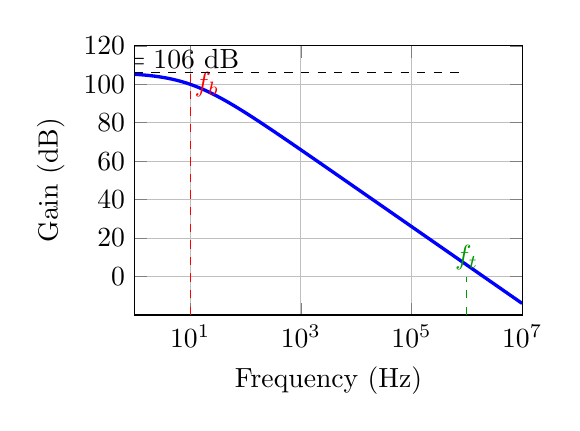
\begin{tikzpicture}
            \begin{axis}[
                width=6.5cm, height=5cm,
                xlabel={Frequency (Hz)},
                ylabel={Gain (dB)},
                xmode=log,
                domain=1:10000000,
                grid=both,
                xmin=1, xmax=10000000,
                ymin=-20, ymax=120,
                ytick={0, 20, 40, 60, 80, 100, 120},
            ]
            % Open-loop gain
            \addplot[blue, very thick, samples=200] {106 - 20*log10(1 + x/10)};
            
            % Annotations
            \draw[dashed, red] (axis cs:10,-20) -- (axis cs:10,106);
            \node[red, rotate=0] at (axis cs:20,100) {$f_b$};
            
            \draw[dashed, green! 60! black] (axis cs:1000000,-20) -- (axis cs:1000000,0);
            \node[green! 60!black] at (axis cs:1000000,10) {$f_t$};
            
            % DC gain line
            \draw[dashed] (axis cs:1,106) -- (axis cs:1000000,106);
            \node at (axis cs:3,112) {$A_0 = 106$ dB};
            
            \end{axis}
        \end{tikzpicture}
        \caption{Typical 741 open-loop response}
        \end{figure}
        
    \end{columns}
    
\end{frame}

\begin{frame}{Gain-Bandwidth Product}
    
    \begin{columns}[t]
    \column{0.48\textwidth}
        \textbf{Unity-Gain Frequency} $f_t$:
        
        Frequency where $|A(f_t)| = 1$ (0 dB):
        \[
        f_t = A_0 \cdot f_b
        \]
        
        \vspace{0.3cm}
        
        \textbf{Gain-Bandwidth Product (GBW)}:
        
        For frequencies $f \gg f_b$:
        \[
        |A(f)| \cdot f = A_0 \cdot f_b = f_t = \text{constant}
        \]
        
        \vspace{0.5cm}
        
        \textbf{Example - 741}:
        \begin{itemize}
            \item $A_0 = 200{,}000$ (106 dB)
            \item $f_b = 5$ Hz
            \item $f_t = 200{,}000 \times 5 = 1$ MHz
            \item GBW = 1 MHz
        \end{itemize}
        
    \column{0.48\textwidth}
        \textbf{Closed-Loop Bandwidth}:
        
        For closed-loop gain $G$:
        \[
        f_{-3dB} = \frac{f_t}{G}
        \]
        
        \vspace{0.3cm}
        
        \begin{block}{Gain-Bandwidth Tradeoff}
            Higher gain $\rightarrow$ lower bandwidth! 
            \[
            G \times BW = f_t = \text{constant}
            \]
        \end{block}
        
        \vspace{0.3cm}
        
        \textbf{Examples} (741, $f_t = 1$ MHz):
        
        \begin{table}
        \small
        \begin{tabular}{|c|c|}
        \hline
        \textbf{Gain} & \textbf{Bandwidth} \\
        \hline
        1 & 1 MHz \\
        10 & 100 kHz \\
        100 & 10 kHz \\
        1000 & 1 kHz \\
        \hline
        \end{tabular}
        \end{table}
        
    \end{columns}
    
\end{frame}

\begin{frame}{Closed-Loop Frequency Response}
    
    \begin{columns}[t]
    \column{0.48\textwidth}
        \textbf{Non-Inverting Amplifier}:
        
        \begin{figure}[htb]
        \centering
        \begin{circuitikz}[scale=0.85]
            % Op-amp
            \draw (0,0) node[op amp, yscale=1.3] (opamp) {};
            
            % Input
            \draw (opamp.+) to[short, -o] ++(-0.8,0) node[left] {$v_{in}$};
            
            % Feedback network
            \draw (opamp.out) to[short, *-] ++(0.5,0) coordinate (out) to[short, -o] ++(0.5,0) node[right] {$v_{out}$};
            \draw (out) -- ++(0,1) to[R, l=$R_f$] ++(-2.5,0) coordinate (fb);
            \draw (fb) to[R, l=$R_i$] (fb |- 0,-1.5) node[ground] {};
            \draw (fb) -- (opamp.-);
        \end{circuitikz}
        \caption{Non-inverting amplifier}
        \end{figure}
        
        \vspace{0.3cm}
        
        \textbf{Ideal Gain}:
        \[
        G = 1 + \frac{R_f}{R_i}
        \]
        
        \textbf{3-dB Bandwidth}: 
        \[
        f_{-3dB} = \frac{f_t}{G}
        \]
        
    \column{0.48\textwidth}
        \textbf{Frequency Response for Different Gains}:
        
        \begin{figure}[htb]
        \centering
        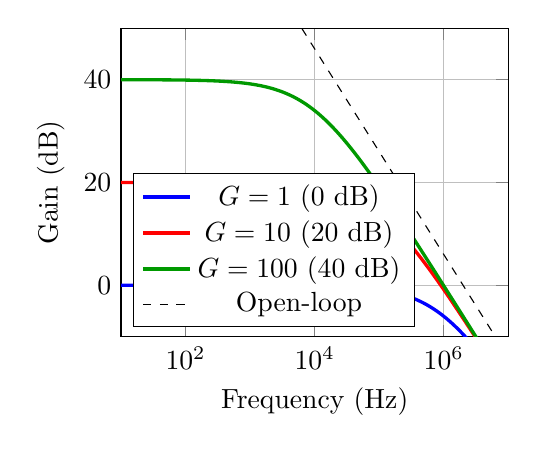
\begin{tikzpicture}
            \begin{axis}[
                width=6.5cm, height=5.5cm,
                xlabel={Frequency (Hz)},
                ylabel={Gain (dB)},
                xmode=log,
                domain=10:10000000,
                grid=both,
                xmin=10, xmax=10000000,
                ymin=-10, ymax=50,
                legend pos=south west,
            ]
            % G = 1
            \addplot[blue, very thick, samples=200] {-20*log10(1 + x/1000000)};
            \addlegendentry{$G = 1$ (0 dB)}
            
            % G = 10
            \addplot[red, very thick, samples=200] {20 - 20*log10(1 + x/100000)};
            \addlegendentry{$G = 10$ (20 dB)}
            
            % G = 100
            \addplot[green! 60!black, very thick, samples=200] {40 - 20*log10(1 + x/10000)};
            \addlegendentry{$G = 100$ (40 dB)}
            
            % Open-loop
            \addplot[black, dashed, samples=200] {106 - 20*log10(1 + x/10)};
            \addlegendentry{Open-loop}
            
            \end{axis}
        \end{tikzpicture}
        \caption{Closed-loop response for various gains}
        \end{figure}
        
    \end{columns}
    
\end{frame}

\begin{frame}{Phase Margin and Stability}

    \begin{columns}[t]
    \column{0.48\textwidth}
    \textbf{Phase Margin (PM)}:

    Amount of additional phase shift (beyond $-180^\circ$) at unity-gain frequency before instability:
    \[
    PM = 180^\circ + \phi(f_t)
    \]

    \vspace{0.3cm}

    \textbf{Stability Criteria}:
    \begin{itemize}
    \item PM $> 45^\circ$: stable, good damping
    \item PM $\approx 60^\circ$: optimal (typical design)
    \item PM $< 30^\circ$: marginal, may oscillate
    \item PM $\leq 0^\circ$: unstable
    \end{itemize}

    \vspace{0.5cm}

    \begin{block}{Compensation}
    Internally compensated op-amps (like 741) have built-in compensation for unity-gain stability.
    \end{block}

    \column{0.48\textwidth}
    \textbf{Bode Plot - Phase Response}:

    \begin{figure}
    \centering
    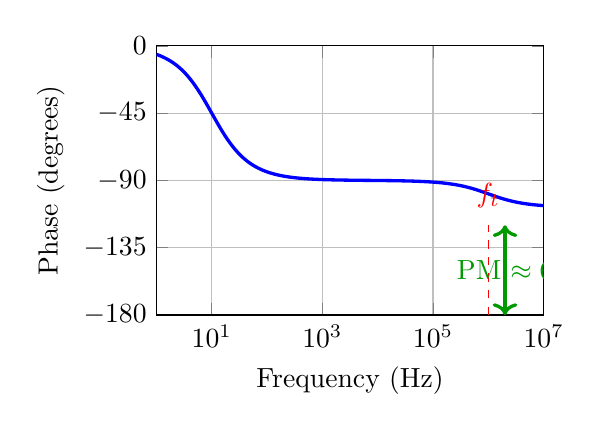
\begin{tikzpicture}
    \begin{axis}[
    width=6.5cm, height=5cm,
    xlabel={Frequency (Hz)},
    ylabel={Phase (degrees)},
    xmode=log,
    domain=1:10000000,
    grid=both,
    xmin=1, xmax=10000000,
    ymin=-180, ymax=0,
    ytick={0, -45, -90, -135, -180},
    ]
    % Phase response (illustrative)
    \addplot[blue, very thick, samples=200] {-atan(x/10) - 0.2*atan(x/1000000)};

    % Unity-gain frequency
    \draw[dashed, red] (axis cs:1000000,-180) -- (axis cs:1000000,-120);
    \node[red] at (axis cs:1000000,-100) {$f_t$};

    % Phase margin annotation
    \draw[<->, green!60!black, very thick] (axis cs:2000000,-180) -- (axis cs:2000000,-120);
    \node[green!60!black] at (axis cs:3500000,-150) {PM $\approx 60^\circ$};

    \end{axis}
    \end{tikzpicture}
    \caption{Phase response showing phase margin}
    \end{figure}

    \end{columns}
\end{frame}

\section{Small Signal Analysis}

\begin{frame}{Small Signal AC Model}
    
    \begin{columns}[t]
    \column{0.48\textwidth}
        \textbf{Frequency-Dependent Model}:
        
        \begin{figure}[htb]
        \centering
        \begin{circuitikz}[scale=0.9]
            % Input terminals
            \draw (0,1) to[short, o-] (1,1) node[above] {$v_+$};
            \draw (0,-1) to[short, o-] (1,-1) node[below] {$v_-$};
            
            % Input impedance
            \draw (1,1) to[R, l=$R_{in}$] (1,-1);
            
            % VCVS
            \draw (3,0) node[circle, draw, thick, minimum size=1.2cm] (vcvs) {$A(f) v_d$};
            \draw (1,1) -- (vcvs.120);
            \draw (1,-1) -- (vcvs.240);
            
            % Output impedance and terminal
            \draw (vcvs.0) to[R, l=$R_{out}$] (5.5,0) to[short, -o] (6,0) node[right] {$v_{out}$};
            
            % Ground reference
            \draw (3,-1.5) node[ground] {} -- (vcvs.270);
            
            \node at (2,-2.5) {$v_d = v_+ - v_-$};
        \end{circuitikz}
        \caption{Small-signal AC model}
        \end{figure}
        
        \vspace{0.3cm}
        
        \textbf{Frequency-Dependent Gain}:
        \[
        A(f) = \frac{A_0}{1 + jf/f_b}
        \]
        
    \column{0.48\textwidth}
        \textbf{Typical Parameter Values}:
        
        \vspace{0.3cm}
        
        \begin{table}
        \small
        \renewcommand{\arraystretch}{1.5}
        \begin{tabular}{|l|c|}
        \hline
        \textbf{Parameter} & \textbf{Typical (741)} \\
        \hline
        $R_{in}$ & 2 M$\Omega$ \\
        $R_{out}$ & 75 $\Omega$ \\
        $A_0$ & 200,000 V/V \\
        $f_b$ & 5 Hz \\
        $f_t$ & 1 MHz \\
        \hline
        \end{tabular}
        \end{table}
        
        \vspace{0.5cm}
        
        \textbf{Analysis Steps}:
        \begin{enumerate}
            \item Replace op-amp with AC model
            \item Apply frequency-dependent $A(f)$
            \item Solve for transfer function
            \item Determine bandwidth from $|H(f)|$
        \end{enumerate}
        
    \end{columns}
    
\end{frame}

\begin{frame}{Closed-Loop Gain Derivation}
    
    \begin{columns}[t]
    \column{0.48\textwidth}
        \textbf{Non-Inverting Amplifier Analysis}:
        
        \begin{figure}[htb]
        \centering
        \begin{circuitikz}[scale=0.75]
            \draw (0,0) node[op amp, yscale=1.3] (opamp) {};
            \draw (opamp.+) to[short, -o] ++(-0.8,0) node[left] {$v_{in}$};
            \draw (opamp.out) to[short, *-] ++(0.5,0) coordinate (out) to[short, -o] ++(0.5,0) node[right] {$v_{out}$};
            \draw (out) -- ++(0,1) to[R, l=$R_f$] ++(-2.5,0) coordinate (fb);
            \draw (fb) to[R, l=$R_i$] (fb |- 0,-1.5) node[ground] {};
            \draw (fb) -- (opamp.-);
            
            % Label nodes
            \node[blue] at (opamp.- |- 0,1.3) {$v_-$};
            \node[blue] at (opamp.+ |- 0,-1.3) {$v_+$};
        \end{circuitikz}
        \end{figure}
        
        \vspace{0.3cm}
        
        \textbf{Feedback factor}:
        \[
        \beta = \frac{R_i}{R_i + R_f}
        \]
        
        \textbf{Ideal closed-loop gain}:
        \[
        G_{ideal} = \frac{1}{\beta} = 1 + \frac{R_f}{R_i}
        \]
        
    \column{0.48\textwidth}
        \textbf{Actual Closed-Loop Gain}: 
        
        With finite open-loop gain $A(f)$:
        \[
        G(f) = \frac{v_{out}}{v_{in}} = \frac{A(f)}{1 + A(f)\beta}
        \]
        
        \vspace{0.3cm}
        
        Substituting $A(f) = A_0/(1 + jf/f_b)$:
        \[
        G(f) = \frac{G_{ideal}}{1 + jf/f_{-3dB}}
        \]
        
        where the 3-dB frequency is: 
        \[
        f_{-3dB} = f_b(1 + A_0\beta) \approx A_0 \beta f_b = \frac{f_t}{G_{ideal}}
        \]
        
        \vspace{0.5cm}
        
        \begin{block}{Key Result}
            Negative feedback: 
            \begin{itemize}
                \item Reduces gain from $A_0$ to $G$
                \item Increases bandwidth by factor $(1 + A_0\beta)$
                \item Product $G \times BW = f_t$ remains constant
            \end{itemize}
        \end{block}
        
    \end{columns}
    
\end{frame}

\begin{frame}{Example:  Bandwidth Calculation}
    
    \textbf{Problem}:  Design a non-inverting amplifier with gain of 20 using a 741 op-amp ($f_t = 1$ MHz). Find the bandwidth.
    
    \vspace{0.5cm}
    
    \begin{columns}[t]
    \column{0.48\textwidth}
        \textbf{Given}:
        \begin{itemize}
            \item Desired gain: $G = 20$
            \item Op-amp: 741 with $f_t = 1$ MHz
        \end{itemize}
        
        \vspace{0.3cm}
        
        \textbf{Design}:
        \[
        G = 1 + \frac{R_f}{R_i} = 20
        \]
        \[
        \frac{R_f}{R_i} = 19
        \]
        
        Choose $R_i = 1$ k$\Omega$, then: 
        \[
        R_f = 19 \text{ k}\Omega
        \]
        
    \column{0.48\textwidth}
        \textbf{Bandwidth}:
        \[
        f_{-3dB} = \frac{f_t}{G} = \frac{1 \text{ MHz}}{20} = 50 \text{ kHz}
        \]
        
        \vspace{0.5cm}
        
        \textbf{Verification}:
        \[
        G \times BW = 20 \times 50 \text{ kHz} = 1 \text{ MHz} = f_t \quad \checkmark
        \]
        
        \vspace{0.5cm}
        
        \begin{alertblock}{Conclusion}
            The amplifier will have a flat gain of 20 (26 dB) from DC up to 50 kHz, then roll off at -20 dB/decade.
        \end{alertblock}
        
    \end{columns}
    
\end{frame}

\section{Slew Rate}

\begin{frame}{Slew Rate:   Large Signal Limitation}
    
    \begin{columns}[t]
    \column{0.48\textwidth}
        \textbf{Definition}:
        
        \textbf{Slew Rate (SR)} is the maximum rate of change of the output voltage: 
        \[
        SR = \left|\frac{dv_{out}}{dt}\right|_{max} \quad \text{(V/}\mu\text{s)}
        \]
        
        \vspace{0.3cm}
        
        \textbf{Physical Cause}:
        \begin{itemize}
            \item Limited internal charging current
            \item Compensation capacitor charging time
            \item Transistor saturation
        \end{itemize}
        
        \vspace{0.5cm}
        
        \textbf{Typical Values}: 
        \begin{itemize}
            \item 741: SR $= 0.5$ V/$\mu$s
            \item TL081: SR $= 13$ V/$\mu$s
            \item LM318: SR $= 70$ V/$\mu$s
            \item LT1819: SR $= 2500$ V/$\mu$s
        \end{itemize}
        
    \column{0.48\textwidth}
        \textbf{Slew Rate Limiting}:
        
        \begin{figure}[htb]
        \centering
        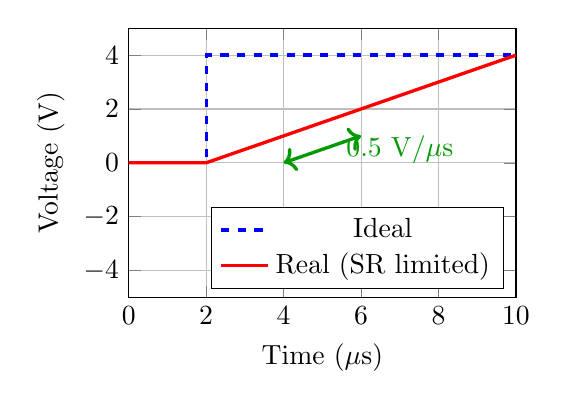
\begin{tikzpicture}
            \begin{axis}[
                width=6.5cm, height=5cm,
                xlabel={Time ($\mu$s)},
                ylabel={Voltage (V)},
                domain=0:10,
                grid=major,
                xmin=0, xmax=10,
                ymin=-5, ymax=5,
                legend pos=south east,
            ]
            % Ideal step response
            \addplot[blue, very thick, dashed] coordinates {
                (0,0) (2,0) (2,4) (10,4)
            };
            \addlegendentry{Ideal}
            
            % Slew-rate limited (SR = 0.5 V/μs)
            \addplot[red, very thick] coordinates {
                (0,0) (2,0) (10,4)
            };
            \addlegendentry{Real (SR limited)}
            
            % Slope annotation
            \draw[<->, green!60!black, very thick] (axis cs:4,0) -- (axis cs:6,1);
            \node[green! 60!black] at (axis cs:7,0.5) {$0.5$ V/$\mu$s};
            
            \end{axis}
        \end{tikzpicture}
        \caption{Step response with slew-rate limiting}
        \end{figure}
        
    \end{columns}
    
\end{frame}

\begin{frame}{Slew Rate and Sinusoidal Signals}
    
    \begin{columns}[t]
    \column{0.48\textwidth}
        \textbf{Sinusoidal Output}:
        
        For $v_{out}(t) = V_p \sin(2\pi f t)$:
        \[
        \frac{dv_{out}}{dt} = 2\pi f V_p \cos(2\pi f t)
        \]
        
        Maximum slope: 
        \[
        \left|\frac{dv_{out}}{dt}\right|_{max} = 2\pi f V_p
        \]
        
        \vspace{0.5cm}
        
        \textbf{No Distortion Condition}:
        \[
        2\pi f V_p \leq SR
        \]
        
        \vspace{0.5cm}
        
        \textbf{Full-Power Bandwidth}:
        
        Maximum frequency for full output swing $V_p$:
        \[
        f_{FP} = \frac{SR}{2\pi V_p}
        \]
        
    \column{0.48\textwidth}
        \textbf{Slew-Rate Distortion}:
        
        \begin{figure}[htb]
        \centering
        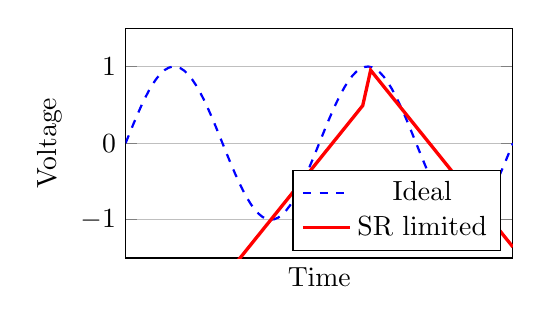
\begin{tikzpicture}
            \begin{axis}[
                width=6.5cm, height=4.5cm,
                xlabel={Time},
                ylabel={Voltage},
                domain=0:4*pi,
                samples=100,
                grid=major,
                xmin=0, xmax=4*pi,
                ymin=-1.5, ymax=1.5,
                xtick=\empty,
                legend pos=south east,
            ]
            % Ideal sinusoid
            \addplot[blue, thick, dashed] {sin(deg(x))};
            \addlegendentry{Ideal}
            
            % Slew-rate limited (triangular)
            \addplot[red, very thick, domain=0:4*pi, samples=50] {
                (x < pi/2) ? 0.5*x : 
                (x < 3*pi/2) ? (1 - 0.5*(x-pi/2)) : 
                (x < 5*pi/2) ? (-1 + 0.5*(x-3*pi/2)) :
                (1 - 0.5*(x-5*pi/2))
            };
            \addlegendentry{SR limited}
            
            \end{axis}
        \end{tikzpicture}
        \caption{Slew-rate distortion of sine wave}
        \end{figure}
        
        \vspace{0.3cm}
        
        \textbf{Example - 741}:
        
        SR $= 0.5$ V/$\mu$s, $V_p = 10$ V: 
        \[
        f_{FP} = \frac{0.5 \times 10^6}{2\pi \times 10} = 7.96 \text{ kHz}
        \]
        
    \end{columns}
    
\end{frame}

% \begin{frame}{Full-Power Bandwidth vs.   Small-Signal Bandwidth}
    
%     \begin{columns}[t]
%     \column{0.48\textwidth}
%         \textbf{Two Different Bandwidths}:
        
%         \vspace{0.3cm}
        
%         \textbf{1. Small-Signal Bandwidth} $f_{-3dB}$:
%         \begin{itemize}
%             \item Determined by GBW product
%             \item $f_{-3dB} = f_t / G$
%             \item Valid for small output swings
%         \end{itemize}
        
%         \vspace{0.5cm}
        
%         \textbf{2. Full-Power Bandwidth} $f_{FP}$:
%         \begin{itemize}
%             \item Determined by slew rate
%             \item $f_{FP} = SR/(2\pi V_p)$
%             \item Valid for large output swings
%         \end{itemize}
        
%         \vspace{0.5cm}
        
%         \begin{block}{Design Rule}
%             Actual usable bandwidth: 
%             \[
%             BW_{actual} = \min(f_{-3dB}, f_{FP})
%             \]
%         \end{block}
        
%     \column{0.48\textwidth}
%         \textbf{Comparison Plot}:
        
%         \begin{figure}[htb]
%         \centering
%         \begin{tikzpicture}
%             \begin{axis}[
%                 width=6.5cm, height=5.5cm,
%                 xlabel={Frequency (Hz)},
%                 ylabel={Max Output (V)},
%                 xmode=log,
%                 domain=10:1000000,
%                 grid=both,
%                 xmin=10, xmax=1000000,
%                 ymin=0, ymax=15,
%                 legend pos=north east,
%             ]
%             % Small-signal bandwidth (flat then rolloff at f_-3dB)
%             \addplot[blue, very thick] coordinates {
%                 (10, 10) (50000, 10) (1000000, 0.5)
%             };
%             \addlegendentry{Small-signal limit}
            
%             % Slew-rate limit (1/f characteristic)
%             \addplot[red, very thick, samples=100] {(0.5e6)/(2*pi*x)};
%             \addlegendentry{Slew-rate limit ($f_{FP}$)}
            
%             % Annotations
%             \draw[dashed, green! 60!black] (axis cs:7960,0) -- (axis cs:7960,10);
%             \node[green! 60!black, rotate=90] at (axis cs:10000,5) {$f_{FP} = 8$ kHz};
            
%             \end{axis}
%         \end{tikzpicture}
%         \caption{741:  $G=1$, SR$=0.5$ V/$\mu$s, $f_t=1$ MHz}
%         \end{figure}
        
%         \vspace{0.3cm}
        
%         \textbf{Note}:  For small signals ($V_p < 1$ V), small-signal BW dominates. For large signals ($V_p = 10$ V), SR dominates.
        
%     \end{columns}
    
% \end{frame}

\begin{frame}{Full-Power Bandwidth vs.\ Small-Signal Bandwidth}

    \begin{columns}[t]
    \column{0.48\textwidth}
    \textbf{Two Different Bandwidths}:

    \vspace{0.3cm}

    \textbf{1. Small-Signal Bandwidth} $f_{-3\text{dB}}$:
    \begin{itemize}
    \item Determined by GBW product
    \item $f_{-3\text{dB}} = f_t / G$
    \item Valid for small output swings
    \end{itemize}

    \vspace{0.5cm}

    \textbf{2. Full-Power Bandwidth} $f_{FP}$:
    \begin{itemize}
    \item Determined by slew rate
    \item $f_{FP} = SR/(2\pi V_p)$
    \item Valid for large output swings
    \end{itemize}

    \vspace{0.5cm}

    \begin{block}{Design Rule}
    Actual usable bandwidth:
    \[
    BW_{actual} = \min(f_{-3\text{dB}}, f_{FP})
    \]
    \end{block}

    \column{0.48\textwidth}
    \textbf{Comparison Plot}:

    \begin{figure}
    \centering
    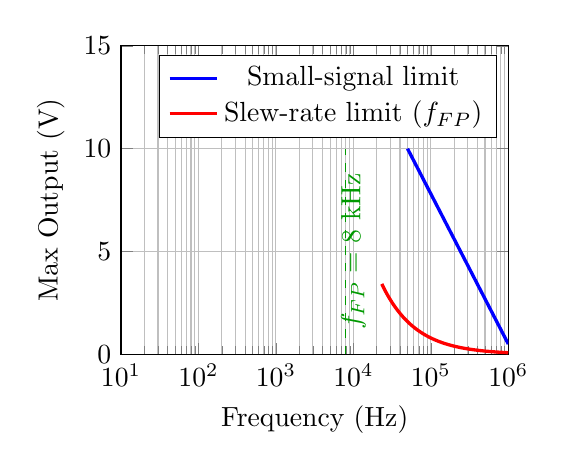
\begin{tikzpicture}
    \begin{axis}[
        width=6.5cm, height=5.5cm,
        xlabel={Frequency (Hz)},
        ylabel={Max Output (V)},
        xmode=log,
        xmin=10, xmax=1000000,
        ymin=0, ymax=15,
        grid=both,
        legend pos=north east,
        unbounded coords=discard,
        restrict x to domain=10:1000000,
        ]
    \addplot[blue, very thick] coordinates {
    (10, 10) (50000, 10) (1000000, 0.5)
    };
    \addlegendentry{Small-signal limit}

    \addplot[red, very thick, samples=200, domain=10:1000000]
  {0.5e6/(2*pi*x)};
    \addlegendentry{Slew-rate limit ($f_{FP}$)}

    \draw[dashed, green!60!black] (axis cs:7960,0) -- (axis cs:7960,10);
    \node[green!60!black, rotate=90] at (axis cs:10000,5) {$f_{FP} = 8$ kHz};

    \end{axis}
    \end{tikzpicture}
    \caption{741: $G=1$, SR$=0.5$ V/$\mu$s, $f_t=1$ MHz}
    \end{figure}

    \vspace{0.3cm}

    \textbf{Note}: For small signals ($V_p < 1$ V), small-signal BW dominates. For large signals ($V_p = 10$ V), SR dominates.

    \end{columns}
\end{frame}

\begin{frame}{Settling Time and Rise Time}
    
    \begin{columns}[t]
    \column{0.48\textwidth}
        \textbf{Settling Time} $t_s$:
        
        Time for output to reach and stay within a specified error band (typically $\pm 0.1\%$ or $\pm 0.01\%$) of final value. 
        
        \vspace{0.3cm}
        
        \begin{figure}[htb]
        \centering
        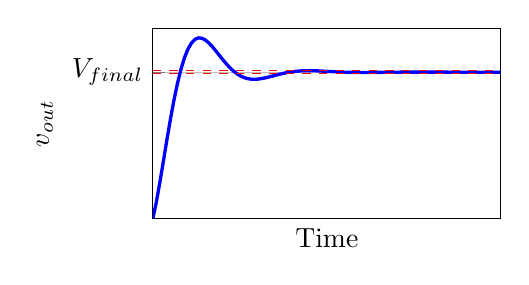
\begin{tikzpicture}
            \begin{axis}[
                width=6cm, height=4cm,
                xlabel={Time},
                ylabel={$v_{out}$},
                domain=0:10,
                samples=100,
                grid=major,
                xmin=0, xmax=10,
                ymin=0, ymax=1.3,
                xtick=\empty,
                ytick={1},
                yticklabels={$V_{final}$},
            ]
            % Step response with overshoot
            \addplot[blue, very thick] {1 - exp(-x)*cos(deg(2*x))};
            
            % Error bands
            \draw[dashed, red] (axis cs: 0,0.99) -- (axis cs:10,0.99);
            \draw[dashed, red] (axis cs:0,1.01) -- (axis cs:10,1.01);
            
            % Settling time
            \draw[<->, green!60!black, very thick] (axis cs:0,-0.1) -- (axis cs:6,-0.1);
            \node[green!60!black] at (axis cs:3,-0.25) {$t_s$};
            
            \end{axis}
        \end{tikzpicture}
        \caption{Settling time to $\pm 1\%$ band}
        \end{figure}
        
    \column{0.48\textwidth}
        \textbf{Rise Time} $t_r$:
        
        Time for output to rise from 10% to 90% of final value.
        
        \vspace{0.3cm}
        
        \textbf{Relationship to Bandwidth}:
        \[
        t_r \approx \frac{0.35}{f_{-3dB}}
        \]
        
        \vspace{0.5cm}
        
        \textbf{Example - Unity-Gain Buffer (741)}:
        
        $f_{-3dB} = f_t = 1$ MHz: 
        \[
        t_r = \frac{0.35}{1 \text{ MHz}} = 0.35\,\mu\text{s} = 350 \text{ ns}
        \]
        
        \vspace{0.5cm}
        
        \begin{alertblock}{Application Note}
            For fast settling: 
            \begin{itemize}
                \item Choose op-amp with high $f_t$
                \item Minimize closed-loop gain
                \item Ensure adequate phase margin
            \end{itemize}
        \end{alertblock}
        
    \end{columns}
    
\end{frame}

\section{Other Important Specifications}

\begin{frame}{Common-Mode Rejection Ratio (CMRR)}
    
    \begin{columns}[t]
    \column{0.48\textwidth}
        \textbf{Definition}:
        
        Ratio of differential gain to common-mode gain:
        \[
        CMRR = \frac{A_d}{A_{cm}} = \frac{|A(v_+ - v_-)|}{|A(v_{cm})|}
        \]
        
        Usually expressed in dB:
        \[
        CMRR_{dB} = 20\log_{10}(CMRR)
        \]
        
        \vspace{0.5cm}
        
        \textbf{Typical Values}: 
        \begin{itemize}
            \item 741:  CMRR $= 90$ dB
            \item OP07: CMRR $= 110$ dB
            \item TL081: CMRR $= 86$ dB
        \end{itemize}
        
        \vspace{0.3cm}
        
        \textbf{Ideal}:  CMRR $= \infty$ (perfect rejection)
        
    \column{0.48\textwidth}
        \textbf{Effect of Finite CMRR}:
        
        Common-mode input $v_{cm}$ appears as:
        \[
        v_{error} = \frac{v_{cm}}{CMRR}
        \]
        
        \vspace{0.3cm}
        
        \textbf{Example}:
        
        $v_{cm} = 5$ V, CMRR $= 90$ dB $= 31{,}623$: 
        \[
        v_{error} = \frac{5}{31{,}623} = 158\,\mu\text{V}
        \]
        
        \vspace{0.5cm}
        
        \textbf{Frequency Dependence}:
        
        \begin{figure}[htb]
        \centering
        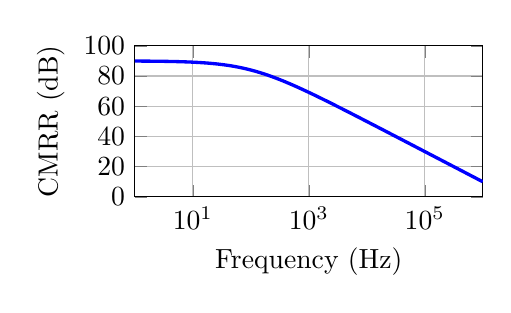
\begin{tikzpicture}
            \begin{axis}[
                width=6cm, height=3.5cm,
                xlabel={Frequency (Hz)},
                ylabel={CMRR (dB)},
                xmode=log,
                domain=1:1000000,
                grid=both,
                xmin=1, xmax=1000000,
                ymin=0, ymax=100,
            ]
            \addplot[blue, very thick, samples=100] {90 - 20*log10(1 + x/100)};
            \end{axis}
        \end{tikzpicture}
        \caption{CMRR decreases with frequency}
        \end{figure}
        
    \end{columns}
    
\end{frame}

\begin{frame}{Power Supply Rejection Ratio (PSRR)}
    
    \begin{columns}[t]
    \column{0.48\textwidth}
        \textbf{Definition}:
        
        Measure of how well op-amp rejects power supply variations:
        \[
        PSRR = \frac{\Delta V_{supply}}{\Delta V_{os}}
        \]
        
        Usually expressed in dB:
        \[
        PSRR_{dB} = 20\log_{10}(PSRR)
        \]
        
        \vspace{0.5cm}
        
        \textbf{Typical Values}: 
        \begin{itemize}
            \item 741: PSRR $= 80$ dB ($+$ supply)
            \item OP07: PSRR $= 110$ dB
            \item TL081: PSRR $= 80$ dB
        \end{itemize}
        
        \vspace{0.3cm}
        
        \textbf{Ideal}: PSRR $= \infty$ (perfect rejection)
        
    \column{0.48\textwidth}
        \textbf{Effect of Finite PSRR}:
        
        Ripple on supply $\Delta V_{supply}$ appears as offset:
        \[
        V_{os,induced} = \frac{\Delta V_{supply}}{PSRR}
        \]
        
        \vspace{0.3cm}
        
        \textbf{Example}: 
        
        100 mV ripple, PSRR $= 80$ dB $= 10{,}000$:
        \[
        V_{os,induced} = \frac{100\text{ mV}}{10{,}000} = 10\,\mu\text{V}
        \]
        
        \vspace{0.5cm}
        
        \begin{block}{Power Supply Design}
            For low-noise applications:
            \begin{itemize}
                \item Use well-regulated supplies
                \item Add bypass capacitors (0.1 $\mu$F ceramic + 10 $\mu$F electrolytic)
                \item Keep supply lines short
                \item Use high-PSRR op-amps
            \end{itemize}
        \end{block}
        
    \end{columns}
    
\end{frame}

\begin{frame}{Input and Output Impedances (Real)}
    
    \begin{columns}[t]
    \column{0.48\textwidth}
        \textbf{Input Impedance}:
        
        \textbf{Differential input impedance}:
        \begin{itemize}
            \item BJT input (741): $R_{in} \approx 2$ M$\Omega$
            \item JFET input (TL081): $R_{in} \approx 10^{12}$ $\Omega$
            \item CMOS input:  $R_{in} \approx 10^{13}$ $\Omega$
        \end{itemize}
        
        \vspace{0.3cm}
        
        \textbf{Common-mode input impedance}:
        \begin{itemize}
            \item Usually much higher
            \item Typically in G$\Omega$ range
        \end{itemize}
        
        \vspace{0.5cm}
        
        \begin{block}{Effect on Source Loading}
            For source impedance $R_s$:
            \[
            \frac{v_{in,actual}}{v_{source}} = \frac{R_{in}}{R_{in} + R_s}
            \]
            
            Rule:  Use $R_s \ll R_{in}/100$ for $<1\%$ error
        \end{block}
        
    \column{0.48\textwidth}
        \textbf{Output Impedance}: 
        
        \textbf{Open-loop}:  $R_{out} \approx 50-100$ $\Omega$ (typical)
        
        \vspace{0.3cm}
        
        \textbf{Closed-loop} (with feedback):
        \[
        R_{out,CL} = \frac{R_{out}}{1 + A\beta}
        \]
        
        For large loop gain $A\beta$:
        \[
        R_{out,CL} \approx \frac{R_{out}}{A\beta} \ll 1\,\Omega
        \]
        
        \vspace{0.5cm}
        
        \textbf{Maximum Output Current}:
        \begin{itemize}
            \item 741: $I_{out,max} \approx \pm 25$ mA
            \item TL081: $I_{out,max} \approx \pm 20$ mA
            \item High-current op-amps: up to $\pm 100$ mA
                \end{itemize}
        
        \vspace{0.3cm}
        
        \begin{alertblock}{Load Considerations}
            Minimum load resistance: 
            \[
            R_L > \frac{V_{out,max}}{I_{out,max}}
            \]
        \end{alertblock}
        
    \end{columns}
    
\end{frame}

\begin{frame}{Output Voltage Swing Limitations}
    
    \begin{columns}[t]
    \column{0.48\textwidth}
        \textbf{Output Swing vs. Supply}:
        
        Output cannot reach supply rails:
        \[
        V_{out,min} = -V_{EE} + V_{sat}
        \]
        \[
        V_{out,max} = +V_{CC} - V_{sat}
        \]
        
        where $V_{sat}$ is the saturation voltage.
        
        \vspace{0.5cm}
        
        \textbf{Typical Saturation Voltages}:
        \begin{itemize}
            \item 741: $V_{sat} \approx 2$ V
            \item TL081: $V_{sat} \approx 1.5$ V
            \item Rail-to-rail op-amps: $V_{sat} \approx 50$ mV
        \end{itemize}
        
    \column{0.48\textwidth}
        \textbf{Example - 741 with $\pm 15$ V supplies}:
        
        \[
        V_{out,max} = +15 - 2 = +13 \text{ V}
        \]
        \[
        V_{out,min} = -15 + 2 = -13 \text{ V}
        \]
        
        Output swing: $\pm 13$ V (not $\pm 15$ V!)
        
        \vspace{0.5cm}
        
        \begin{figure}[htb]
        \centering
        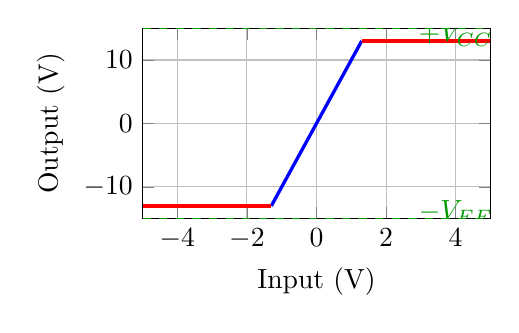
\begin{tikzpicture}
            \begin{axis}[
                width=6cm, height=4cm,
                xlabel={Input (V)},
                ylabel={Output (V)},
                domain=-5:5,
                grid=major,
                xmin=-5, xmax=5,
                ymin=-15, ymax=15,
            ]
            % Linear region
            \addplot[blue, very thick, domain=-1.3:1.3] {10*x};
            
            % Saturation regions
            \addplot[red, very thick, domain=-5:-1.3] {-13};
            \addplot[red, very thick, domain=1.3:5] {13};
            
            % Supply rails
            \draw[dashed, green! 60! black] (axis cs:-5,15) -- (axis cs:5,15);
            \draw[dashed, green!60!black] (axis cs:-5,-15) -- (axis cs:5,-15);
            \node[green!60!black] at (axis cs: 4,14) {$+V_{CC}$};
            \node[green!60!black] at (axis cs:4,-14) {$-V_{EE}$};
            
            \end{axis}
        \end{tikzpicture}
        \caption{Output clipping (saturation)}
        \end{figure}
        
    \end{columns}
    
\end{frame}

\section{Op-Amp Selection Guide}

\begin{frame}{Choosing the Right Op-Amp}
    
    \begin{table}
    \centering
    \renewcommand{\arraystretch}{1.6}
    \small
    \begin{tabular}{|l|l|l|}
    \hline
    \textbf{Application} & \textbf{Key Specs} & \textbf{Recommended} \\
    \hline
    \hline
    General purpose & Low cost, moderate specs & 741, LM324, TL081 \\
    \hline
    Precision DC amplifier & Low $V_{OS}$, low drift & OP07, OP177, LT1013 \\
    \hline
    High-speed & High SR, high $f_t$ & LM318, THS4031, AD8099 \\
    \hline
    Audio & Low noise, good THD & NE5532, OPA2134, LM4562 \\
    \hline
    Low power & Low supply current & TLV2371, LMC7101, MAX4236 \\
    \hline
    High input impedance & JFET/CMOS input & TL081, CA3140, LMC6482 \\
    \hline
    Single supply & Rail-to-rail I/O & LM358, LMV321, MCP6002 \\
    \hline
    Instrumentation & High CMRR, low noise & INA128, AD620, LT1167 \\
    \hline
    \end{tabular}
    \end{table}
    
    \vspace{0.5cm}
    
    \begin{block}{Selection Process}
        \begin{enumerate}
            \item Identify critical requirements (bandwidth, accuracy, power, etc.)
            \item Check datasheets for specs
            \item Verify operating conditions (supply voltage, temperature range)
            \item Consider cost and availability
            \item Simulate or prototype to verify
        \end{enumerate}
    \end{block}
    
\end{frame}

\begin{frame}{Comparison of Common Op-Amps}
    
    \begin{table}
    \centering
    \renewcommand{\arraystretch}{1.5}
    \tiny
    \begin{tabular}{|l|c|c|c|c|c|c|}
    \hline
    \textbf{Part} & \textbf{$A_0$ (dB)} & \textbf{$f_t$ (MHz)} & \textbf{SR (V/$\mu$s)} & \textbf{$V_{OS}$ (mV)} & \textbf{$I_B$} & \textbf{Type} \\
    \hline
    \hline
    741 & 106 & 1 & 0.5 & 1-5 & 80 nA & BJT, general \\
    \hline
    LM324 & 100 & 1 & 0.5 & 2-7 & 45 nA & BJT, quad, single supply \\
    \hline
    TL081 & 106 & 3 & 13 & 3-15 & 50 pA & JFET, high $Z_{in}$ \\
    \hline
    OP07 & 120 & 0.6 & 0.3 & 0.025-0.075 & 2 nA & BJT, precision \\
    \hline
    OP177 & 126 & 0.6 & 0.3 & 0.01-0.025 & 0.5 nA & BJT, ultra-precision \\
    \hline
    LM318 & 100 & 15 & 70 & 2-10 & 150 nA & BJT, high-speed \\
    \hline
    THS4031 & 110 & 100 & 370 & 0.5 & 10 $\mu$A & BJT, very high-speed \\
    \hline
    NE5532 & 100 & 10 & 9 & 0.5-4 & 200 nA & BJT, low-noise audio \\
    \hline
    LMC6482 & 106 & 1.5 & 1.1 & 0.4-1.5 & 2 fA & CMOS, rail-to-rail \\
    \hline
    CA3140 & 100 & 4.5 & 9 & 2-15 & 10 pA & BiMOS, high $Z_{in}$ \\
    \hline
    \end{tabular}
    \end{table}
    
    \vspace{0.3cm}
    
    \begin{alertblock}{Design Tradeoffs}
        \begin{itemize}
            \item \textbf{Precision vs. Speed}: High precision op-amps often have lower bandwidth
            \item \textbf{Input Type}: BJT (low $V_{OS}$), JFET (low $I_B$), CMOS (ultra-low $I_B$)
            \item \textbf{Power vs. Performance}: Lower power $\rightarrow$ lower speed/drive capability
        \end{itemize}
    \end{alertblock}
    
\end{frame}

\section{Summary}

\begin{frame}{Summary:  Real Op-Amp Specifications}
    
    \begin{columns}[t]
    \column{0.48\textwidth}
        \textbf{DC Specifications}:
        \begin{itemize}
            \item Open-loop gain: $A_0$ (finite, not infinite)
            \item Input offset voltage: $V_{OS}$
            \item Input bias current: $I_B$
            \item Input offset current: $I_{OS}$
            \item Temperature drift: $dV_{OS}/dT$, $dI_B/dT$
        \end{itemize}
        
        \vspace{0.5cm}
        
        \textbf{Frequency Response}:
        \begin{itemize}
            \item Open-loop gain: $A(f) = A_0/(1 + jf/f_b)$
            \item Unity-gain frequency: $f_t$
            \item Gain-bandwidth product: $G \times BW = f_t$
            \item Phase margin (stability)
        \end{itemize}
        
    \column{0.48\textwidth}
        \textbf{Dynamic Limitations}:
        \begin{itemize}
            \item Slew rate: SR (V/$\mu$s)
            \item Full-power bandwidth: $f_{FP} = SR/(2\pi V_p)$
            \item Settling time, rise time
            \item Output swing limitations
        \end{itemize}
        
        \vspace{0.5cm}
        
        \textbf{Other Specifications}:
        \begin{itemize}
            \item CMRR (common-mode rejection)
            \item PSRR (power supply rejection)
            \item Input impedance: $R_{in}$
            \item Output impedance:  $R_{out}$
            \item Maximum output current
        \end{itemize}
        
    \end{columns}
    
    \vspace{0.5cm}
    
    \begin{alertblock}{Design Approach}
        \textbf{Always check datasheets! } Match op-amp specs to application requirements.  Don't over-specify (cost), don't under-specify (performance).
    \end{alertblock}
    
\end{frame}

\begin{frame}{Key Formulas Reference}
    
    \begin{table}
    \centering
    \renewcommand{\arraystretch}{2.0}
    \small
    \begin{tabular}{|l|c|}
    \hline
    \textbf{Parameter} & \textbf{Formula} \\
    \hline
    \hline
    Open-loop gain (AC) & $A(f) = \dfrac{A_0}{1 + jf/f_b}$ \\
    \hline
    Unity-gain frequency & $f_t = A_0 \cdot f_b$ \\
    \hline
    Closed-loop bandwidth & $f_{-3dB} = \dfrac{f_t}{G_{closed}}$ \\
    \hline
    Gain-bandwidth product & $G \times BW = f_t = \text{constant}$ \\
    \hline
    Full-power bandwidth & $f_{FP} = \dfrac{SR}{2\pi V_p}$ \\
    \hline
    Rise time & $t_r \approx \dfrac{0.35}{f_{-3dB}}$ \\
    \hline
    Max slew rate & $SR = \left|\dfrac{dv_{out}}{dt}\right|_{max}$ \\
    \hline
    Offset error (amplified) & $V_{out,error} = V_{OS} \cdot G$ \\
    \hline
    \end{tabular}
    \end{table}
    
\end{frame}

\begin{frame}{Practice Problem 1}
    
    \textbf{Given}:  A non-inverting amplifier using a 741 op-amp ($f_t = 1$ MHz, SR $= 0.5$ V/$\mu$s) with $R_i = 1$ k$\Omega$ and $R_f = 99$ k$\Omega$. 
    
    \vspace{0.5cm}
    
    \textbf{Find}:
    \begin{enumerate}
        \item[(a)] The ideal closed-loop gain
        \item[(b)] The small-signal bandwidth
        \item[(c)] The maximum output voltage swing at 10 kHz without slew-rate distortion
        \item[(d)] The full-power bandwidth for $V_{out,p} = 10$ V
    \end{enumerate}
    
    \vspace{0.5cm}
    
    \textbf{Hints}:
    \begin{itemize}
        \item $G = 1 + R_f/R_i$
        \item $f_{-3dB} = f_t/G$
        \item $SR = 2\pi f V_p$ (for undistorted sine wave)
        \item $f_{FP} = SR/(2\pi V_p)$
    \end{itemize}
    
\end{frame}

\ifshowsolutions
\begin{frame}{Practice Problem 1 Solution}
    
    \textbf{Given}: $R_i = 1$ k$\Omega$, $R_f = 99$ k$\Omega$, $f_t = 1$ MHz, SR $= 0.5$ V/$\mu$s
    
    \vspace{0.3cm}
    
    \textbf{(a) Closed-loop gain}:
    \[
    G = 1 + \frac{R_f}{R_i} = 1 + \frac{99\text{ k}\Omega}{1\text{ k}\Omega} = 1 + 99 = 100
    \]
    
    \textbf{(b) Small-signal bandwidth}:
    \[
    f_{-3dB} = \frac{f_t}{G} = \frac{1\text{ MHz}}{100} = 10\text{ kHz}
    \]
    
    \textbf{(c) Max output at 10 kHz}: 
    
    For no slew-rate distortion:  $SR = 2\pi f V_p$
    \[
    V_p = \frac{SR}{2\pi f} = \frac{0.5 \times 10^6\text{ V/s}}{2\pi \times 10{,}000\text{ Hz}} = 7.96\text{ V}
    \]
    
    \textbf{(d) Full-power bandwidth for 10 V}:
    \[
    f_{FP} = \frac{SR}{2\pi V_p} = \frac{0.5 \times 10^6}{2\pi \times 10} = 7.96\text{ kHz}
    \]
    
\end{frame}
\fi

\begin{frame}{Practice Problem 2}
    
    \textbf{Given}: An inverting amplifier with gain of $-50$ using an OP07 op-amp: 
    \begin{itemize}
        \item $A_0 = 1{,}000{,}000$ (120 dB)
        \item $V_{OS} = 50$ $\mu$V at 25$\circ$C
        \item $dV_{OS}/dT = 0.3$ $\mu$V/$\circ$C
        \item $I_B = 2$ nA
        \item $R_i = 10$ k$\Omega$
    \end{itemize}
    
    \vspace{0.5cm}
    
    \textbf{Find}:
    \begin{enumerate}
        \item[(a)] $R_f$ for the desired gain
        \item[(b)] Output offset voltage due to $V_{OS}$ at 25$\circ$C
        \item[(c)] Additional output error due to $I_B$ (worst case)
        \item[(d)] Total output offset at 70$\circ$C
    \end{enumerate}
    
\end{frame}

\ifshowsolutions
\begin{frame}{Practice Problem 2 Solution}

    \textbf{(a) Feedback resistor}:

    For inverting amplifier: $G = -R_f/R_i = -50$
    \[
    R_f = 50 \times R_i = 50 \times 10\,\text{k}\Omega = 500\,\text{k}\Omega
    \]

    \textbf{(b) Output offset at $25^\circ\mathrm{C}$}:

    Inverting config acts like non-inverting for offset: $|G| = 1 + R_f/R_i = 51$
    \[
    V_{out,\text{offset}} = V_{OS} \times 51 = 50\,\mu\text{V} \times 51 = 2.55\,\text{mV}
    \]

    \textbf{(c) Error from bias current}:
    \[
    V_{\text{error},IB} = I_B \times R_f = 2\,\text{nA} \times 500\,\text{k}\Omega = 1\,\text{mV}
    \]

    \textbf{(d) Total offset at $70^\circ\mathrm{C}$}:

    \[
    \Delta T = 70 - 25 = 45^\circ\mathrm{C}
    \]
    \[
    V_{OS,70} = 50\,\mu\text{V} + (0.3\,\mu\text{V}/^\circ\mathrm{C}) \times 45^\circ\mathrm{C}
    = 63.5\,\mu\text{V}
    \]
    \[
    V_{out,\text{total}} = (63.5\,\mu\text{V} \times 51) + 1\,\text{mV}
    = 3.24\,\text{mV} + 1\,\text{mV} = 4.24\,\text{mV}
    \]

\end{frame}
\fi

\begin{frame}{Practice Problem 3}
    
    \textbf{Scenario}: You need to amplify a 1 kHz sine wave from 100 mV peak to 5 V peak with less than 1\% distortion.
    
    \vspace{0.5cm}
    
    \textbf{Given two op-amp options}:
    \begin{itemize}
        \item \textbf{Option A}: $f_t = 1$ MHz, SR $= 0.5$ V/$\mu$s
        \item \textbf{Option B}: $f_t = 10$ MHz, SR $= 10$ V/$\mu$s
    \end{itemize}
    
    \vspace{0.5cm}
    
    \textbf{Questions}:
    \begin{enumerate}
        \item[(a)] What gain is required? 
        \item[(b)] Is Option A suitable?  Check both bandwidth and slew rate.
        \item[(c)] Is Option B suitable? Check both bandwidth and slew rate.
        \item[(d)] Which would you choose and why?
    \end{enumerate}
    
\end{frame}

\ifshowsolutions
\begin{frame}{Practice Problem 3 Solution}
    
    \textbf{(a) Required gain}:
    \[
    G = \frac{V_{out,p}}{V_{in,p}} = \frac{5\text{ V}}{0.1\text{ V}} = 50
    \]
    
    \textbf{(b) Option A - Check}:
    
    Bandwidth: $f_{-3dB} = f_t/G = 1\text{ MHz}/50 = 20\text{ kHz} > 1\text{ kHz}$ \gooditem
    
    Slew rate: Required SR $= 2\pi f V_p = 2\pi \times 1000 \times 5 = 31.4\text{ kV/s} = 0.031\text{ V/}\mu\text{s}$
    
    Available SR $= 0.5\text{ V/}\mu\text{s} > 0.031\text{ V/}\mu\text{s}$ \gooditem
    
    \textbf{Option A is suitable! }
    
    \vspace{0.3cm}
    
    \textbf{(c) Option B - Check}:
    
    Bandwidth: $f_{-3dB} = 10\text{ MHz}/50 = 200\text{ kHz} \gg 1\text{ kHz}$ \gooditem
    
    Slew rate: Available $= 10\text{ V/}\mu\text{s} \gg 0.031\text{ V/}\mu\text{s}$ \gooditem
    
    \textbf{Option B is also suitable (with margin)!}
    
    \vspace{0.3cm}
    
    \textbf{(d) Recommendation}: Choose \textbf{Option A} — adequate performance at likely lower cost.  Option B is over-specified for this application.
    
\end{frame}
\fi

\end{document}